%%%%%%%%%%%%%%%%%%%%%%%%%%%%%%%%%%%%%%%%%%%%%%%%%%%%%%%%%%%%
\documentclass[9pt,            % Schriftgröße {{{
               a4paper,         % A4
               landscape,
               halfparskip,
               oneside,         % Einseitig
               DIV34,           % Papiergröße
              ]{scrartcl} %%% }}}
%%%%%%%%%%%%%%%%%%%%%%%%%%%%%%%%%%%%%%%%%%%%%%%%%%%%%%%%%%%%

%%%%%%%%%%%%%%%%%%%%%%%%%%%%%%%%%%%%%%%%%%%%%%%%%%%%%%%%%%%%
%%% Pakete {{{
\usepackage[utf8]{inputenc}         % Umlaute etc.
\usepackage[T1]{fontenc}            % T1-kodierte Fonts
\usepackage{ae,aecompl}             % Kodierung für PDF
\usepackage{ngerman}                % Deutsche Trennungen,
                                    % dt. Begriffe
\usepackage{setspace}               % Single- oder Onehalfspacing
\setcounter{tocdepth}{4}            % 4 Hirarchien im Inhaltsv.
\usepackage{times}                  % Times als Schrift
\usepackage{amsmath,amssymb,amstext}% Mathematische Symbole
\usepackage{exscale}                % Skalierung von Summen-c und Int.-zeichen
\usepackage{url}                    % Darstellung von URLs
\usepackage{calc}

%%% Optional, je nach Dokument
% \usepackage{listings}             % Quelltext-Listings
% \usepackage{units}                % Technische Units
% \usepackage{psfrag}               % Ersetzts PS-Schriften
  \usepackage{color}                % Farben in LaTeX
% \usepackage{floatflt}             % Textumflossene Bilder...
% \usepackage{picins}               % Textumflossene Bilder
  \usepackage{textcomp}             % Spezielle Zeichen
  \usepackage{gensymb}              % Spezielle Zeichen
% \usepackage{eurosym}              % Euro-Symbol
% \usepackage{currvita}             % Befehle für CVs
  \usepackage{ifpdf}                % Wird ein PDF erstellt?

%%% Layout
\usepackage{scrpage2}               % KOMA-Überschriften und -Fußzeilen.
%%% }}}
%%%%%%%%%%%%%%%%%%%%%%%%%%%%%%%%%%%%%%%%%%%%%%%%%%%%%%%%%%%%

%%%%%%%%%%%%%%%%%%%%%%%%%%%%%%%%%%%%%%%%%%%%%%%%%%%%%%%%%%%%
%%% PDF {{{

\ifpdf
  \usepackage[pdftex]{graphicx}
  \DeclareGraphicsExtensions{.pdf}
  \pdfcompresslevel=9
  \usepackage[%
    pdftex=true,
    backref=true,
    colorlinks=true,
    bookmarks=true,
    breaklinks=true,
    linktocpage=true,
    bookmarksopen=false,
    bookmarksnumbered=false,
    pdfpagemode=None
  ]{hyperref}
  \hypersetup{
    pdftitle={},
    pdfauthor={Julius Plenz},
    pdfsubject={},
    pdfcreator={LaTeX2e and pdfLaTeX},
    pdfproducer={},
    pdfkeywords={}
  }
\else
  \usepackage[dvips]{graphicx}
  \DeclareGraphicsExtensions{.eps}
  % \usepackage[%
  %   dvips,
  %   breaklinks=true,
  %   colorlinks=false
  % ]{hyperref}
\fi

%%% }}}
%%%%%%%%%%%%%%%%%%%%%%%%%%%%%%%%%%%%%%%%%%%%%%%%%%%%%%%%%%%%

%%%%%%%%%%%%%%%%%%%%%%%%%%%%%%%%%%%%%%%%%%%%%%%%%%%%%%%%%%%%
%%% Eigene Funktionen {{{
%%% Beispiel:  \bild{200pt}{foo}{That's a foo\ldots}
\newcommand{\bild}[3]{
  \begin{figure}
    \includegraphics[width=#1, keepaspectratio=true]{#2}
    \caption{#3}
    \label{#2}
  \end{figure}
}

%% \floatimg{filename}{caption+label}{r/l}{8cm}
\newcommand{\floatimg}[4]{
  \piccaption{#2}
  \parpic[#3]{\includegraphics[width=#4]{#1}}
}
%%% }}}
%%%%%%%%%%%%%%%%%%%%%%%%%%%%%%%%%%%%%%%%%%%%%%%%%%%%%%%%%%%%

%%%%%%%%%%%%%%%%%%%%%%%%%%%%%%%%%%%%%%%%%%%%%%%%%%%%%%%%%%%%
%%% Pagestyle {{{
% \pagestyle{scrheadings}
% \pagestyle{fancyhdrs}
  \pagestyle{empty}
%%% }}}
%%%%%%%%%%%%%%%%%%%%%%%%%%%%%%%%%%%%%%%%%%%%%%%%%%%%%%%%%%%%

%%%%%%%%%%%%%%%%%%%%%%%%%%%%%%%%%%%%%%%%%%%%%%%%%%%%%%%%%%%%
%%% Seitenkopf- und -Fußzeilen {{{
 \automark[subsection]{section} % \left- und \rightmark bekommen Inhalt
%%% Oben: Links, Mitte, Rechts
 \ihead[]{}
 \chead[]{}
 \ohead[]{}
%%% Unten: Links, Mitte, Rechts
 \ifoot[]{}
 \cfoot[]{}
 \ofoot[]{}
%%% }}}
%%%%%%%%%%%%%%%%%%%%%%%%%%%%%%%%%%%%%%%%%%%%%%%%%%%%%%%%%%%%

\usepackage{tikz}
\usetikzlibrary{shapes,decorations,shadows}

%%%%%%%%%%%%%%%%%%%%%%%%%%%%%%%%%%%%%%%%%%%%%%%%%%%%%%%%%%%%
%%% Sonstiges {{{
% \setlength{\parindent}{17pt}      % Einzug 17pt,
% \setlength{\parskip}{2pt}         % keine Leerzeilen.

% \textwidth      127mm             % Textbreite
% \textheight     235mm             % Texthöhe
% \topmargin     -5mm               % Abstand oben
% \oddsidemargin  7mm               % Abstand Links, onepage

%\onehalfspacing                    % Zeilenabstand: Bei korrektur,
 \singlespacing                     % bei Abgabe

% Punkt- und Komma Abstände bei Tausendern/
% Dezimalzahlen ans deutsche anpassen!
 \mathcode`,="013B
 \mathcode`.="613A

 \setlength{\emergencystretch}{2em} % Notfallsstreckung
 \addtolength{\voffset}{10pt}

% Kommandoänderungen
 \renewcommand{\figurename}{Abb.} % Bildunterschriften: Abb. anstatt Fig.
%\renewcommand*{\cvheadingfont}{\raggedleft\Huge\bfseries} % CV: Überschriften
%%% }}}
%%%%%%%%%%%%%%%%%%%%%%%%%%%%%%%%%%%%%%%%%%%%%%%%%%%%%%%%%%%%

\begin{document}

%%%%%%%%%%%%%%%%%%%%%%%%%%%%%%%%%%%%%%%%%%%%%%%%%%%%%%%%%%%%
%%% Inhalt {{{


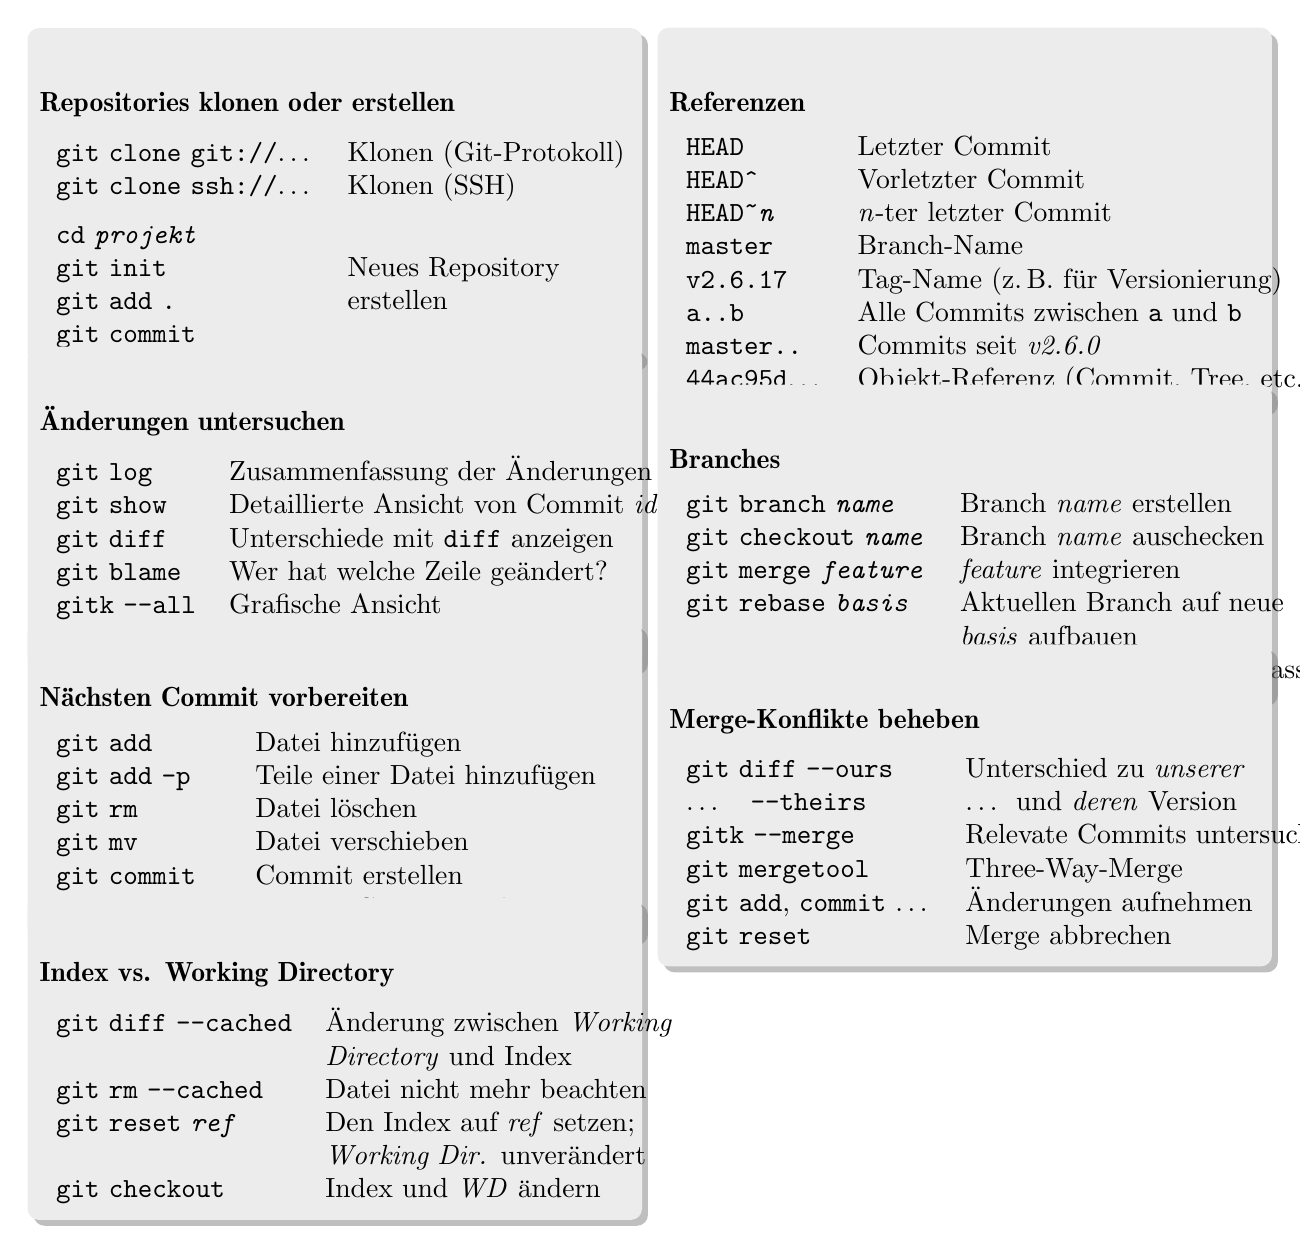
\begin{tikzpicture}
  \draw
  (0,0) node[text width=7.5cm,rounded corners,fill=gray!15,inner sep=1ex,drop shadow]
  {
    \subsubsection*{Repositories klonen oder erstellen}
    \begin{tabular}{ll}
    \texttt{git clone git://}\ldots & Klonen (Git-Protokoll)\\
    \texttt{git clone ssh://}\ldots & Klonen (SSH)
    \vspace*{.2cm}\\
    \texttt{cd \emph{projekt}} & \\
    \texttt{git init} & Neues Repository \\
    \texttt{git add .} & erstellen\\
    \texttt{git commit} &
    \end{tabular}
  }
  ++(0,-1.9cm) node[below,text width=7.5cm,rounded corners,fill=gray!15,inner sep=1ex,drop shadow]
  {
    \subsubsection*{Änderungen untersuchen}
    \begin{tabular}{ll}
    \texttt{git log} & Zusammenfassung der Änderungen\\
    \texttt{git show} & Detaillierte Ansicht von Commit \emph{id}\\
    \texttt{git diff} & Unterschiede mit \texttt{diff} anzeigen\\
    \texttt{git blame} & Wer hat welche Zeile geändert?\\
    \texttt{gitk -{}-all} & Grafische Ansicht\\
    \texttt{tig} & Curses-Frontend für Git
    \end{tabular}
  }
  ++(0,-3.5cm) node[below,text width=7.5cm,rounded corners,fill=gray!15,inner sep=1ex,drop shadow]
  {
    \subsubsection*{Nächsten Commit vorbereiten}
    \begin{tabular}{ll}
    \texttt{git add} & Datei hinzufügen\\
    \texttt{git add -p} & Teile einer Datei hinzufügen\\
    \texttt{git rm} & Datei löschen\\
    \texttt{git mv} & Datei verschieben\\
    \texttt{git commit} & Commit erstellen\\
    \ldots\quad\texttt{-{}-amend} & Letzten Commit verbessern\\
    \end{tabular}
  }
  ++(0,-3.5cm) node[below,text width=7.5cm,rounded corners,fill=gray!15,inner sep=1ex,drop shadow]
  {
    \subsubsection*{Index vs. Working Directory}
    \begin{tabular}{ll}
    \texttt{git diff -{}-cached} & Änderung zwischen \emph{Working}\\
                                 & \emph{Directory} und Index\\
    \texttt{git rm -{}-cached} & Datei nicht mehr beachten\\
    \texttt{git reset \emph{ref}} & Den Index auf \emph{ref} setzen;\\
                                  & \emph{Working Dir.} unverändert\\
    \texttt{git checkout} & Index und \emph{WD} ändern\\
    \end{tabular}
  };
  \draw
  (8cm,-8pt) node[text width=7.5cm,rounded corners,fill=gray!15,inner sep=1ex,drop shadow]
  {
    \subsubsection*{Referenzen}
    \begin{tabular}{ll}
    \texttt{HEAD} & Letzter Commit\\
    \texttt{HEAD\^{}} & Vorletzter Commit\\
    \texttt{HEAD\~{}\emph{n}} & \emph{n}-ter letzter Commit\\
    \texttt{master} & Branch-Name\\
    \texttt{v2.6.17} & Tag-Name (z.\,B. für Versionierung)\\
    \texttt{a..b} & Alle Commits zwischen \texttt{a} und \texttt{b}\\
    \texttt{master..} & Commits seit \emph{v2.6.0}\\
    \texttt{44ac95d}\ldots & Objekt-Referenz (Commit, Tree, etc.)\\
    \end{tabular}
  }
  ++(0,-2.1cm) node[below,text width=7.5cm,rounded corners,fill=gray!15,inner sep=1ex,drop shadow]
  {
    \subsubsection*{Branches}
    \begin{tabular}{ll}
    \texttt{git branch \emph{name}} & Branch \emph{name} erstellen\\
    \texttt{git checkout \emph{name}} & Branch \emph{name} auschecken\\
    \texttt{git merge \emph{feature}} & \emph{feature} integrieren\\
    \texttt{git rebase \emph{basis}} & Aktuellen Branch auf neue \\
                                     & \emph{basis} aufbauen\\
    \ldots\;\texttt{-{}-interactive} & Commits ordnen und anpassen\\
    \end{tabular}
  }
  ++(0,-3.3cm) node[below,text width=7.5cm,rounded corners,fill=gray!15,inner sep=1ex,drop shadow]
  {
    \subsubsection*{Merge-Konflikte beheben}
    \begin{tabular}{ll}
    \texttt{git diff -{}-ours} & Unterschied zu \emph{unserer}\\
    \ldots\quad\texttt{-{}-theirs} & \ldots{} und \emph{deren} Version\\
    \texttt{gitk -{}-merge} & Relevate Commits untersuchen\\
    \texttt{git mergetool} & Three-Way-Merge\\
    \texttt{git add}, \texttt{commit} \ldots & Änderungen aufnehmen\\
    \texttt{git reset} & Merge abbrechen\\
    \end{tabular}
  }
  ;
\end{tikzpicture}
% Box für eigene Tips (später platzieren) TODO
% \draw[fill=gray!10,dashed,rounded corners] (4cm,-14cm) rectangle (6cm,-16cm);

% Als Visualisierung brauchbar?
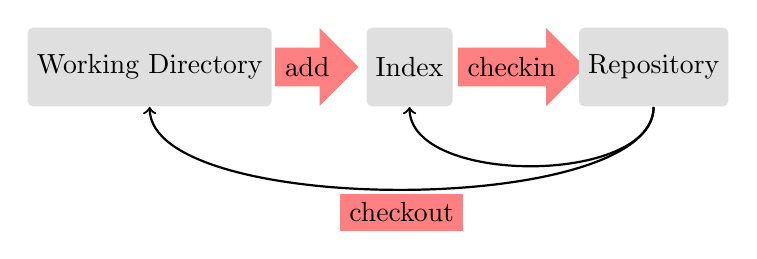
\begin{tikzpicture}
\draw
  (0,0)     node[rounded corners=2pt,fill=gray!25,minimum height=1cm] (w) {Working Directory}
++(2,0)     node[single arrow,fill=red!50] {add}
++(1.3,0)   node[rounded corners=2pt,fill=gray!25,minimum height=1cm] (i) {Index}
++(1.3,0)   node[single arrow,fill=red!50] {checkin}
++(1.8,0)   node[rounded corners=2pt,fill=gray!25,minimum height=1cm] (r) {Repository}
;
\draw[->,thick] (r.south) .. controls +(0,-1) and +(0,-1) .. (i.south);
\draw[->,thick] (r.south) .. controls +(0,-1.4) and +(0,-1.4) .. node[fill=red!50,below=1pt]{checkout} (w.south);
\end{tikzpicture}


%%% }}}
%%%%%%%%%%%%%%%%%%%%%%%%%%%%%%%%%%%%%%%%%%%%%%%%%%%%%%%%%%%%

\end{document}

%%% vim:set fdm=marker:
